\documentclass[../Kamil_Kowalewski_Main.tex]{subfiles}

\begin{document} {

    W~czasach niesamowicie szybkiego rozwoju technologii, szczególnie tych związanych
    z~informatyką, możliwość dokonywania różnych operacji w~sposób zdalny poprzez
    wykorzystanie komputera jest niezwykle wygodne oraz pożądane przez obywateli wysoko
    rozwiniętych państw. Jedną z~takich operacji są zakupy online na portalach
    ogłoszeniowych.

    \section{Problematyka}
    \label{chapter1:wstep:problematyka} {
        Problematyka dotycząca rekomendacji oraz określania wiarygodności ofert na
        portalach ogłoszeniowych jest rozległa i~zdecydowanie nie jest trywialna. Ze
        względu na mnogość portali oraz ofert, które są umieszczane na nich, użytkownicy
        często mają do podjęcia naprawdę trudne decyzje w~czasie zakupu. Jest to
        spowodowane głównie określeniem, które z~ofert są godne zaufania, a~które nie.
        Dla człowieka jest to proces żmudny oraz długotrwały co zaprzecza podstawowym
        założeniom handlu w~internecie, który ma być szybki i~wygodny. Całe szczęście
        istnieją sposoby na automatyzację procesu weryfikacji ofert. Niniejsza praca
        magisterska ma za zadanie przedstawić nową metodę i~porównać ją z~dostępnymi
        rozwiązaniami.

        Celem potwierdzenia bardzo szybkiego rozwoju rynku e-commerce został
        zamieszczony wykres na rysunku \ref{fig:chapter1:wstep:problematyka:sales},
        przedstawiający sprzedaż w~zależności od roku. Jak łatwo zauważyć
        w~przeciągu 7~lat -~od roku 2014 do roku 2021 sprzedaż wzrosła o~ponad 3,5 raza.
        Poprzez znak \textit{*} zostały oznaczone prognozowane wartości dla przyszłych
        lat. Jak widać, w~2025 roku prognozowany jest wzrost o~5,5 raza w~stosunku do 2014
        roku.

        \begin{figure}[H]
            \centering
            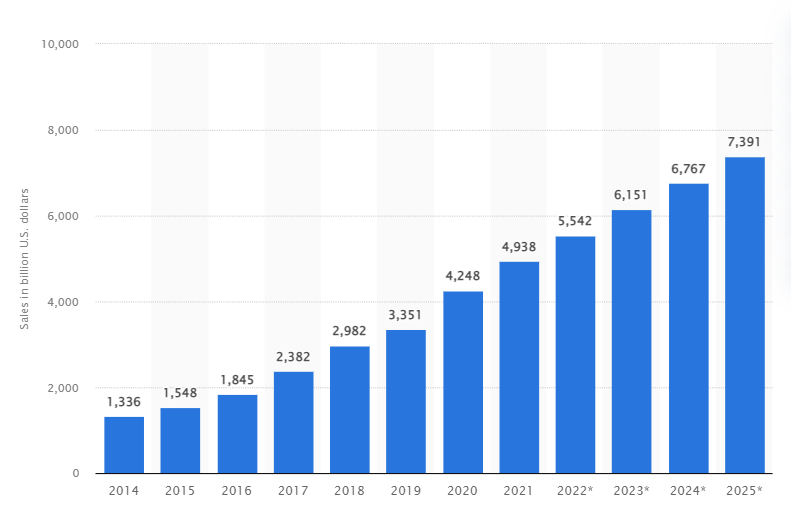
\includegraphics
            [width=0.8\textwidth,keepaspectratio]
            {img/chapter1/e_commerce_sales.png}
            \caption
            [Sprzedaż detaliczna e-commerce na całym świecie w latach 2014-2025
                \cite{website:e_commerce_sales}]
            {Sprzedaż detaliczna e-commerce na całym świecie w latach 2014-2025
                \cite{website:e_commerce_sales}}
            \label{fig:chapter1:wstep:problematyka:sales}
        \end{figure}
    }

    \section{Cel i założenia projektu}
    \label{chapter1:wstep:cel} {
        Celem niniejszej pracy magisterskiej było opracowanie autorskiej metody do
        określania wiarygodności ofert. W~zakres prac można również włączyć analizę
        metod dostępnych w~literaturze naukowej, implementację jednej z~nich
        i~dokonanie porównania z~zaproponowaną metodą przez autora niniejszej pracy.
    }

    \section{Definicje pojęć}
    \label{chapter1:wstep:definicje} {

        \textbf{Portal ogłoszeniowy} - aplikacja webowa umieszczona w sieci
        Internet, która jest powszechnie dostępna. Zapewnia ona możliwość tworzenia
        konta użytkownika, które jest wymagana do sprzedaży i zakupu przedmiotów.
        Do przeglądania nie jest wymagane korzystanie z konta użytkownika.
        Przedmiot jest wystawiany przez sprzedającego natomiast zakupu dokonuje
        kupujący. Po zatwierdzeniu łączy ich swoista umowa kupna-sprzedaży, z
        której dwie strony są zmuszone się wywiązać.

        \textbf{Oferta} - jeden z podstawowych obiektów. Zawiera ona w sobie
        sprzedawany produkt, osobę, która go sprzedaję, liczbę sztuk, cenę, opinie
        innych użytkowników, którzy już dokonali jego zakupu i mieli ochotę wyrazić
        opinię na temat transakcji oraz produktu.

        \textbf{Nieuczciwy sprzedawca} - sprzedawca, który umyślnie
        wprowadza w błąd kupującego poprzez podanie nieprawdziwych informacji na
        temat sprzedawanego produktu. W ten sposób oferta może stać się
        niewiarygodna.

    }

    \section{Układ pracy}
    \label{chapter1:wstep:uklad} {
        Pierwszy rozdział stanowi wstęp do tematyki portali ogłoszeniowych,
        rekomendacji ofert oraz określania ich wiarygodności. Drugi rozdział prezentuje
        przegląd literatury naukowej dostępnej w~chwili opracowywania metody oraz
        tworzenia niniejszej pracy magisterskiej. Następny w~kolejności rozdział
        przedstawia autorską metodę oceny wiarygodności ofert opracowaną oraz hipotezę
        badawczą, która w~kolejnych rozdziałach będzie weryfikowana. Następnym,
        czwartym z~kolei rozdziałem jest dotyczący środowiska eksperymentalnego, opisu
        implementacji autorskiej metody oraz całego programu wykorzystującego tę metodę.
        Piąty rozdział przedstawia wyniki przeprowadzonych eksperymentów oraz ich
        wizualizację. Ostatni rozdział zawiera podsumowanie i~wnioski całej pracy
        magisterskiej oraz weryfikację postawionej hipotezy badawczej.
    }

}
\end{document}
